\documentclass[11pt,a4paper]{article}

% --- Essential Packages ---
\usepackage[utf8]{inputenc}
\usepackage[margin=1in]{geometry}
\usepackage{amsmath,amssymb,amsfonts}
\usepackage{booktabs}
\usepackage{graphicx}
\usepackage{tabularx}
\usepackage{multirow}
\usepackage{caption}
\usepackage{subcaption}
\usepackage{hyperref}
\usepackage{microtype}
\usepackage{setspace}
\usepackage{mathptmx} % Times New Roman equivalent
\usepackage{enumitem}
\usepackage[authoryear]{natbib}

\hypersetup{
    colorlinks=true,
    linkcolor=blue,
    citecolor=blue,
    urlcolor=blue
}

\onehalfspacing

\title{\textbf{\Large Deciphering Non-linear and Dynamic Valuation of Hotel Attributes: \\ An Explainable Machine Learning (XAI) Framework for Online Travel Agencies}}

\author{
    \textbf{Md Naim Molla}\textsuperscript{1,*} \\[0.5em]
    \small \textsuperscript{1}Department of Computer Science and Engineering / Business Analytics \\
    \small \textsuperscript{*}Corresponding author: \texttt{naim@example.com}
}

\date{\today}

\begin{document}

\maketitle

\begin{abstract}
\noindent Traditional hedonic pricing models in hospitality economics rely predominantly on linear or log-linear econometric regressions, which inherently constrain their ability to capture complex feature interactions, asymmetric price elasticities, and non-linear threshold effects. Conversely, modern machine learning algorithms offer superior predictive performance but have historically functioned as uninterpretable ``black boxes,'' limiting their utility for economic theory and policy formulation. 

To bridge this methodological gap, this study develops an \textbf{Explainable Machine Learning (XAI)} framework using \textbf{Tree-SHAP (Shapley Additive exPlanations)} grounded in cooperative game theory to unpack the implicit attribute valuations of hotel accommodations. Using a large-scale panel dataset of \textbf{4,426 verified hotel observations} collected across \textbf{34 global destinations} spanning four distinct market typologies (\textit{Metropolitan Hubs, Luxury/Resort Markets, Regional Leisure Destinations, and Emerging Tourism Hubs}) and three sequential booking lead-time horizons (30, 60, and 90 days), we systematically benchmark parametric econometric models against non-linear ensemble learners.

Empirical results from rigorous 5-fold cross-validation reveal that tree-based ensemble architectures (\textbf{Random Forest $R^2 = 0.8807$, LightGBM $R^2 = 0.8799$}) substantially outperform the classical linear Hedonic OLS baseline ($R^2 = 0.7714$), reducing Mean Absolute Percentage Error (MAPE) from $36.37\%$ to $23.74\%$. Tree-SHAP attribution demonstrates that online reputation signals (\texttt{review\_count} and \texttt{review\_score\_overall}) exert higher marginal pricing power than conventional star-rating classifications, validating Signaling Theory in digital platforms characterized by information asymmetry. Furthermore, dynamic panel analysis reveals a steep non-linear \textbf{$+37.9\%$ dynamic price surge} as lead time narrows from 90 to 30 days, providing empirical evidence of algorithmic revenue management. Finally, cross-market typology comparisons establish that amenity shadow prices are context-dependent: basic bundling (e.g., free breakfast at $50.6\%$) dominates emerging markets, whereas metropolitan hubs command a $+293\%$ location premium driven by spatial rent density. We conclude with actionable policy recommendations for municipal transit planning, smart tourism bed taxes, and hotel revenue management.

\vspace{0.8em}
\noindent \textbf{Keywords:} Hedonic Pricing; Machine Learning; Explainable AI (XAI); Tree-SHAP; Online Travel Agencies (OTAs); Dynamic Revenue Management; Signaling Theory.
\end{abstract}

\newpage

\section{Introduction}

The rapid digitalization of the global hospitality ecosystem, spearheaded by Online Travel Agencies (OTAs) such as Booking.com, Expedia, and Agoda, has fundamentally transformed how accommodation prices are determined, displayed, and consumed \citep{viglia2016, sun2022}. In contemporary digital marketplaces, hotel room rates are no longer static seasonal quotes; rather, they function as high-frequency dynamic prices generated by algorithmic revenue management systems that react continuously to consumer search patterns, remaining inventory, competitor positioning, and multidimensional reputation signals \citep{li2019}.
The rapid digitalization of the global hospitality ecosystem, spearheaded by Online Travel Agencies (OTAs) such as Booking.com, Expedia, and Agoda, has fundamentally transformed how accommodation prices are determined, displayed, and consumed \citep{abrate2016, viglia2016}. In contemporary digital marketplaces, hotel room rates are no longer static seasonal quotes; rather, they function as high-frequency dynamic prices generated by algorithmic revenue management systems that react continuously to consumer search patterns, remaining inventory, competitor positioning, and multidimensional reputation signals \citep{li2018}.

For over half a century, the empirical valuation of lodging attributes has been anchored in \citet{rosen1974} and \citet{lancaster1966} \textbf{Hedonic Pricing Theory}. Under this paradigm, a heterogeneous commodity---such as a hotel room---is decomposed into a bundle of utility-bearing constituent attributes (e.g., star tier, spatial proximity to city centers, swimming pools, high-speed WiFi, breakfast bundling), where the market price reflects the sum of the implicit shadow prices of these characteristics \citep{espinet2003, thrane2007}.

Despite its widespread adoption, classical hedonic pricing literature suffers from a fundamental \textbf{methodological dilemma}:
\begin{enumerate}[leftmargin=*]
    \item \textbf{Parametric Econometric Models (OLS, Box-Cox, Spatial Error Models):} While offering transparent coefficient interpretability, classical linear and log-linear regressions impose rigid functional forms. They assume monotonic, symmetric returns to quality improvements and fail to capture multi-way feature interactions, threshold ``tipping points,'' and extreme multicollinearity among collinear amenities \citep{wang2017}.
    \item \textbf{Machine Learning Ensembles (XGBoost, Random Forest, Neural Networks):} While machine learning algorithms excel at capturing high-order non-linearities and optimizing predictive accuracy ($R^2 > 0.85$), they have historically operated as opaque ``black boxes'' that obscure the marginal economic willingness-to-pay (WTP) necessary for economic theory, managerial strategy, and municipal policy design \citep{sanchez2020, giacalone2023}.
    \item \textbf{Machine Learning Ensembles (XGBoost, Random Forest, Neural Networks):} While machine learning algorithms excel at capturing high-order non-linearities and optimizing predictive accuracy ($R^2 > 0.85$), they have historically operated as opaque ``black boxes'' that obscure the marginal economic willingness-to-pay (WTP) necessary for economic theory, managerial strategy, and municipal policy design \citep{sanchez2019, wang2017}.
\end{enumerate}

Furthermore, empirical literature in hospitality analytics remains constrained by two pervasive shortcomings:
\begin{itemize}[leftmargin=*]
    \item \textbf{Single-City Bias:} Over $80\%$ of published studies analyze an isolated metropolitan area (e.g., only London, New York, or Madrid), ignoring whether attribute valuations remain robust across differing tourism market structures (e.g., resort destinations vs. emerging markets).
    \item \textbf{Static Snapshot Bias:} The majority of existing studies scrape data at a single static point in time, failing to capture dynamic lead-time pacing and algorithmic yield adjustments as check-in dates approach.
\end{itemize}

To address these foundational gaps, this paper establishes a unified \textbf{Explainable Artificial Intelligence (XAI)} framework for hospitality economics. Utilizing \textbf{Tree-SHAP (Shapley Additive exPlanations)} grounded in cooperative game theory \citep{lundberg2017}, we reconcile predictive power with rigorous econometric interpretability. 

Specifically, this study answers four central research questions:
\begin{itemize}[leftmargin=*]
    \item \textbf{RQ1:} To what extent do non-linear machine learning ensembles outperform classical linear hedonic specifications in predicting room rates across diverse global markets?
    \item \textbf{RQ2:} When decomposed game-theoretically, what are the primary structural, reputational, spatial, and dynamic drivers of hotel pricing power on digital OTAs?
    \item \textbf{RQ3:} How do amenity shadow prices and bundling strategies vary across distinct tourism market typologies (\textit{Metropolitan Hubs, Luxury/Resort Markets, Regional Leisure Destinations, and Emerging Tourism Markets})?
    \item \textbf{RQ4:} How does algorithmic dynamic pricing evolve across sequential booking horizons (30-day, 60-day, and 90-day lead times), and what are the implications for consumer welfare and municipal tourism policy?
\end{itemize}

\section{Theoretical Framework \& Hypotheses}

\subsection{Hedonic Valuation \& Lancaster's Consumer Theory}
Hedonic pricing theory posits that consumers derive utility not from a good itself, but from the specific characteristics embedded within that good \citep{lancaster1966, rosen1974}. In lodging markets, the observed equilibrium price $P_i$ of hotel property $i$ is formulated as a function of its vector of structural attributes $\mathbf{S}_i$, location and spatial characteristics $\mathbf{L}_i$, physical amenities $\mathbf{A}_i$, reputation signals $\mathbf{R}_i$, and dynamic booking terms $\mathbf{D}_i$:
\begin{equation}
P_i = f(\mathbf{S}_i, \mathbf{L}_i, \mathbf{A}_i, \mathbf{R}_i, \mathbf{D}_i) + \varepsilon_i
\end{equation}
In classical econometrics, the marginal willingness-to-pay (WTP) for attribute $k$ is computed as the partial derivative $\frac{\partial P}{\partial x_k}$. However, in the presence of complex non-linearities and multi-attribute bundling (e.g., a luxury spa providing higher marginal utility when paired with a 5-star brand), classical linear models yield biased and unstable estimates \citep{chen2010, schamel2012}.

\subsection{Signaling Theory and Reputation Capital}
In online booking environments, consumers face significant \textbf{information asymmetry} because they cannot physically inspect hotel quality prior to purchase \citep{spence1973}. Under Signaling Theory, verifiable third-party signals---such as official star classifications, aggregate consumer review ratings, and review volume---act as trust-building mechanisms that reduce perceived transaction risk \citep{viglia2016}. Recent literature indicates that user-generated review metrics have increasingly surpassed official star ratings in dictating pricing power, as consumers perceive peer feedback as more authentic and real-time \citep{moro2023}.
In online booking environments, consumers face significant \textbf{information asymmetry} because they cannot physically inspect hotel quality prior to purchase \citep{spence1973}. Under Signaling Theory, verifiable third-party signals---such as official star classifications, aggregate consumer review ratings, and review volume---act as trust-building mechanisms that reduce perceived transaction risk \citep{viglia2016}. Recent literature indicates that user-generated review metrics have increasingly surpassed official star ratings in dictating pricing power, as consumers perceive peer feedback as more authentic and real-time \citep{moro2018}.

\subsection{Monocentric Spatial Rent Theory}
Rooted in \citet{alonso1964} monocentric urban model, lodging properties situated near central business districts (CBDs), major transit hubs, or natural tourist attractions command substantial spatial rent premiums. As distance from the focal tourism center increases, price decays along a continuous gradient ($\Delta P / \text{km}$) reflecting travel costs and time disutility incurred by tourists \citep{espinet2003, thrane2007}.

\subsection{Research Hypotheses}
Based on the theoretical literature, we formulate four testable hypotheses:
\begin{itemize}[leftmargin=*]
    \item \textbf{$H_1$ (Methodological Superiority):} \textit{Non-linear tree ensemble algorithms (Random Forest, LightGBM, XGBoost) demonstrate statistically superior out-of-sample predictive accuracy and lower percentage error compared to classical linear hedonic OLS models.}
    \item \textbf{$H_2$ (Reputational Preeminence):} \textit{In digital OTA environments, verified consumer reputation signals (\texttt{review\_count} and \texttt{review\_score\_overall}) exhibit higher marginal pricing power than physical star classifications.}
    \item \textbf{$H_3$ (Dynamic Lead-Time Surge):} \textit{Hotel room rates display a statistically significant, non-linear price surge as the booking horizon narrows from 90 days to 30 days before check-in.}
    \item \textbf{$H_4$ (Typological Moderation):} \textit{The implicit shadow prices of physical amenities and bundling strategies are moderated by tourism market typologies, exhibiting higher bundling prevalence in emerging markets and higher land-rent premiums in metropolitan hubs.}
\end{itemize}

\section{Methodology \& Empirical Design}

\subsection{Data Architecture \& Multi-Market Panel Collection}
To ensure robust empirical generalizability and eliminate single-city bias, data was harvested from Booking.com across \textbf{34 major international tourism destinations} located in North America, Europe, the Middle East, East Asia, Southeast Asia, and South Asia. 

To capture dynamic revenue management and lead-time price adjustments, a panel collection architecture was executed across three standardized check-in windows:
\begin{enumerate}
    \item \textbf{Short-Term Horizon (30-Day Lead Time):} Capturing short-lead business and spontaneous leisure demand.
    \item \textbf{Mid-Term Horizon (60-Day Lead Time):} Standard advance holiday booking window.
    \item \textbf{Long-Term Horizon (90-Day Lead Time):} Early-bird promotional baseline.
\end{enumerate}
The final dataset comprises \textbf{$N = 4,426$ verified, non-duplicate property observations} across \textbf{48 operationalized variables}.

\subsection{Operationalization of Variables}
The dependent variable is the net room rate per night in USD (\texttt{price\_net}). To normalize right-skewness and stabilize error variance, the natural log transformation is employed:
\begin{equation}
y_i = \ln(\text{price\_net}_i)
\end{equation}
Independent variables are categorized into five structural vectors:
\begin{enumerate}[leftmargin=*]
    \item \textbf{Structural Attributes ($\mathbf{S}$):} Official star rating (\texttt{star\_rating} 1--5), property category (\texttt{property\_type}), photo volume (\texttt{photo\_count}).
    \item \textbf{Spatial Metrics ($\mathbf{L}$):} Distance to downtown (\texttt{distance\_to\_center\_km}), beachfront access (\texttt{is\_beachfront}), GPS coordinates (\texttt{latitude}, \texttt{longitude}).
    \item \textbf{Reputation \& Service Quality ($\mathbf{R}$):} Overall review rating (\texttt{review\_score\_overall}), total published reviews (\texttt{review\_count}), and seven dimensional sub-scores (\texttt{score\_cleanliness}, \texttt{score\_staff}, \texttt{score\_facilities}, \texttt{score\_comfort}, \texttt{score\_value}, \texttt{score\_location}, \texttt{score\_wifi}).
    \item \textbf{Physical Amenities Matrix ($\mathbf{A}$):} Eleven binary facility indicators (\texttt{has\_swimming\_pool}, \texttt{has\_free\_wifi}, \texttt{has\_parking}, \texttt{has\_air\_conditioning}, \texttt{has\_spa}, \texttt{has\_fitness\_center}, \texttt{has\_restaurant}, \texttt{has\_bar}, \texttt{has\_airport\_shuttle}, \texttt{has\_24h\_front\_desk}, \texttt{pets\_allowed}).
    \item \textbf{Booking Terms \& Dynamic Signals ($\mathbf{D}$):} Cancellation terms (\texttt{free\_cancellation}), breakfast bundle (\texttt{breakfast\_included}), municipal taxes (\texttt{taxes\_and\_charges}), discount depth (\texttt{discount\_pct}), urgency tag (\texttt{rooms\_left\_warning}), lead time (\texttt{lead\_time\_days}), and weekend dummy (\texttt{is\_weekend}).
\end{enumerate}

\subsection{Model Benchmarking Strategy}
To rigorously test $H_1$, we benchmark six algorithms under a standardized \textbf{5-Fold Cross-Validation protocol}:
\begin{enumerate}[leftmargin=*]
    \item \textbf{Hedonic OLS Linear Regression:} Classical parametric benchmark.
    \item \textbf{Ridge Regression ($L_2$ Regularization):}
    \begin{equation}
    \min_{\boldsymbol{\beta}} \left\{ \sum_{i=1}^n \left(y_i - \mathbf{x}_i^T\boldsymbol{\beta}\right)^2 + \lambda \sum_{j=1}^p \beta_j^2 \right\}
    \end{equation}
    \item \textbf{Lasso Regression ($L_1$ Regularization):}
    \begin{equation}
    \min_{\boldsymbol{\beta}} \left\{ \sum_{i=1}^n \left(y_i - \mathbf{x}_i^T\boldsymbol{\beta}\right)^2 + \alpha \sum_{j=1}^p |\beta_j| \right\}
    \end{equation}
    \item \textbf{Random Forest Regressor:} Non-parametric ensemble of 100 decorrelated bagged decision trees \citep{breiman2001}.
    \item \textbf{LightGBM Regressor:} Gradient boosted decision tree framework optimizing leaf-wise split criteria with GOSS and EFB \citep{ke2017}.
    \item \textbf{XGBoost Regressor:} Regularized boosting optimizing a second-order Taylor expansion of the loss function \citep{chen2016}.
\end{enumerate}

\subsection{Game-Theoretic Explainability: Tree-SHAP Formulation}
To extract exact marginal attribute contributions from non-linear ensembles, we implement \textbf{Tree-SHAP} \citep{lundberg2017}. Grounded in cooperative game theory \citep{shapley1953}, the SHAP value $\phi_j(x)$ represents the unique, additive contribution of feature $j$ to the model prediction $f(x)$ relative to the expected base value $E[f(x)]$:
\begin{equation}
f(x) = E[f(x)] + \sum_{j=1}^M \phi_j(x)
\end{equation}
The exact Shapley value for feature $j$ across all possible feature subsets $S \subseteq F \setminus \{j\}$ is:
\begin{equation}
\phi_j(x) = \sum_{S \subseteq F \setminus \{j\}} \frac{|S|!(|F| - |S| - 1)!}{|F|!} \left[ f_x(S \cup \{j\}) - f_x(S) \right]
\end{equation}
Global feature importance is measured as the mean absolute SHAP value:
\begin{equation}
I_j = \frac{1}{n} \sum_{i=1}^n |\phi_j(x_i)|
\end{equation}

\section{Empirical Results}

\subsection{Descriptive Statistics}
Table \ref{tab:desc_stats} reports the descriptive statistics for the complete empirical sample ($N = 4,426$).

\begin{table}[htbp]
\centering
\small
\caption{Descriptive Statistics of Key Empirical Variables ($N = 4,426$)}
\label{tab:desc_stats}
\begin{tabular*}{\textwidth}{@{\extracolsep{\fill}}lrrrrrr@{}}
\toprule
\textbf{Variable} & \textbf{Mean} & \textbf{Std Dev} & \textbf{Min} & \textbf{Median} & \textbf{Max} & \textbf{Skewness} \\
\midrule
\texttt{price\_net} (USD)       & 191.634 & 186.625 & 2.000  & 142.000 & 4439.000 & +4.741 \\
\texttt{log\_price} ($\ln$ USD) & 4.859   & 0.951   & 0.693  & 4.956   & 8.398    & -0.431 \\
\texttt{taxes\_and\_charges}    & 28.388  & 33.632  & 0.000  & 17.000  & 266.000  & +2.650 \\
\texttt{star\_rating}           & 2.564   & 1.750   & 0.000  & 3.000   & 5.000    & -0.460 \\
\texttt{review\_score\_overall} & 8.117   & 1.162   & 1.000  & 8.400   & 10.000   & -2.062 \\
\texttt{review\_count}          & 2493.20 & 3308.84 & 0.000  & 1316.00 & 37613.00 & +2.866 \\
\texttt{distance\_to\_center\_km}& 4.135  & 5.029   & 0.050  & 2.300   & 40.700   & +2.512 \\
\texttt{breakfast\_included}    & 0.221   & 0.415   & 0.000  & 0.000   & 1.000    & +1.342 \\
\texttt{free\_cancellation}     & 0.431   & 0.495   & 0.000  & 0.000   & 1.000    & +0.277 \\
\texttt{is\_beachfront}         & 0.009   & 0.092   & 0.000  & 0.000   & 1.000    & +10.656 \\
\texttt{has\_swimming\_pool}    & 0.054   & 0.225   & 0.000  & 0.000   & 1.000    & +3.968 \\
\texttt{has\_air\_conditioning} & 0.781   & 0.414   & 0.000  & 1.000   & 1.000    & -1.360 \\
\texttt{lead\_time\_days}       & 59.108  & 25.416  & 29.000 & 59.000  & 89.000   & -0.007 \\
\bottomrule
\end{tabular*}
\end{table}

\subsection{Benchmark Performance Comparison (Validation of $H_1$)}
Table \ref{tab:benchmark} reports the 5-fold cross-validation performance across the six model specifications.

\begin{table}[htbp]
\centering
\small
\caption{5-Fold Cross-Validation Model Benchmark Tournament}
\label{tab:benchmark}
\begin{tabular*}{\textwidth}{@{\extracolsep{\fill}}lcccc@{}}
\toprule
\textbf{Model Specification} & \textbf{$R^2$ Score (CV)} & \textbf{RMSE ($\ln$)} & \textbf{MAE ($\ln$)} & \textbf{MAPE (\%)} \\
\midrule
\textbf{1. Random Forest Regressor} & \textbf{0.8807 ($\pm$0.008)} & \textbf{0.3282} & \textbf{0.2235} & \textbf{23.74\%} \\
\textbf{2. LightGBM Regressor}      & \textbf{0.8799 ($\pm$0.007)} & \textbf{0.3293} & \textbf{0.2356} & \textbf{24.66\%} \\
\textbf{3. XGBoost Regressor}       & \textbf{0.8756 ($\pm$0.007)} & \textbf{0.3350} & \textbf{0.2429} & \textbf{25.35\%} \\
4. Ridge Regression                 & 0.7715 ($\pm$0.003)          & 0.4542          & 0.3423          & 36.34\% \\
5. Hedonic OLS (Linear)             & 0.7714 ($\pm$0.003)          & 0.4543          & 0.3424          & 36.37\% \\
6. Lasso Regression                 & 0.7693 ($\pm$0.003)          & 0.4564          & 0.3436          & 36.50\% \\
\bottomrule
\end{tabular*}
\end{table}

\begin{figure}[htbp]
\centering
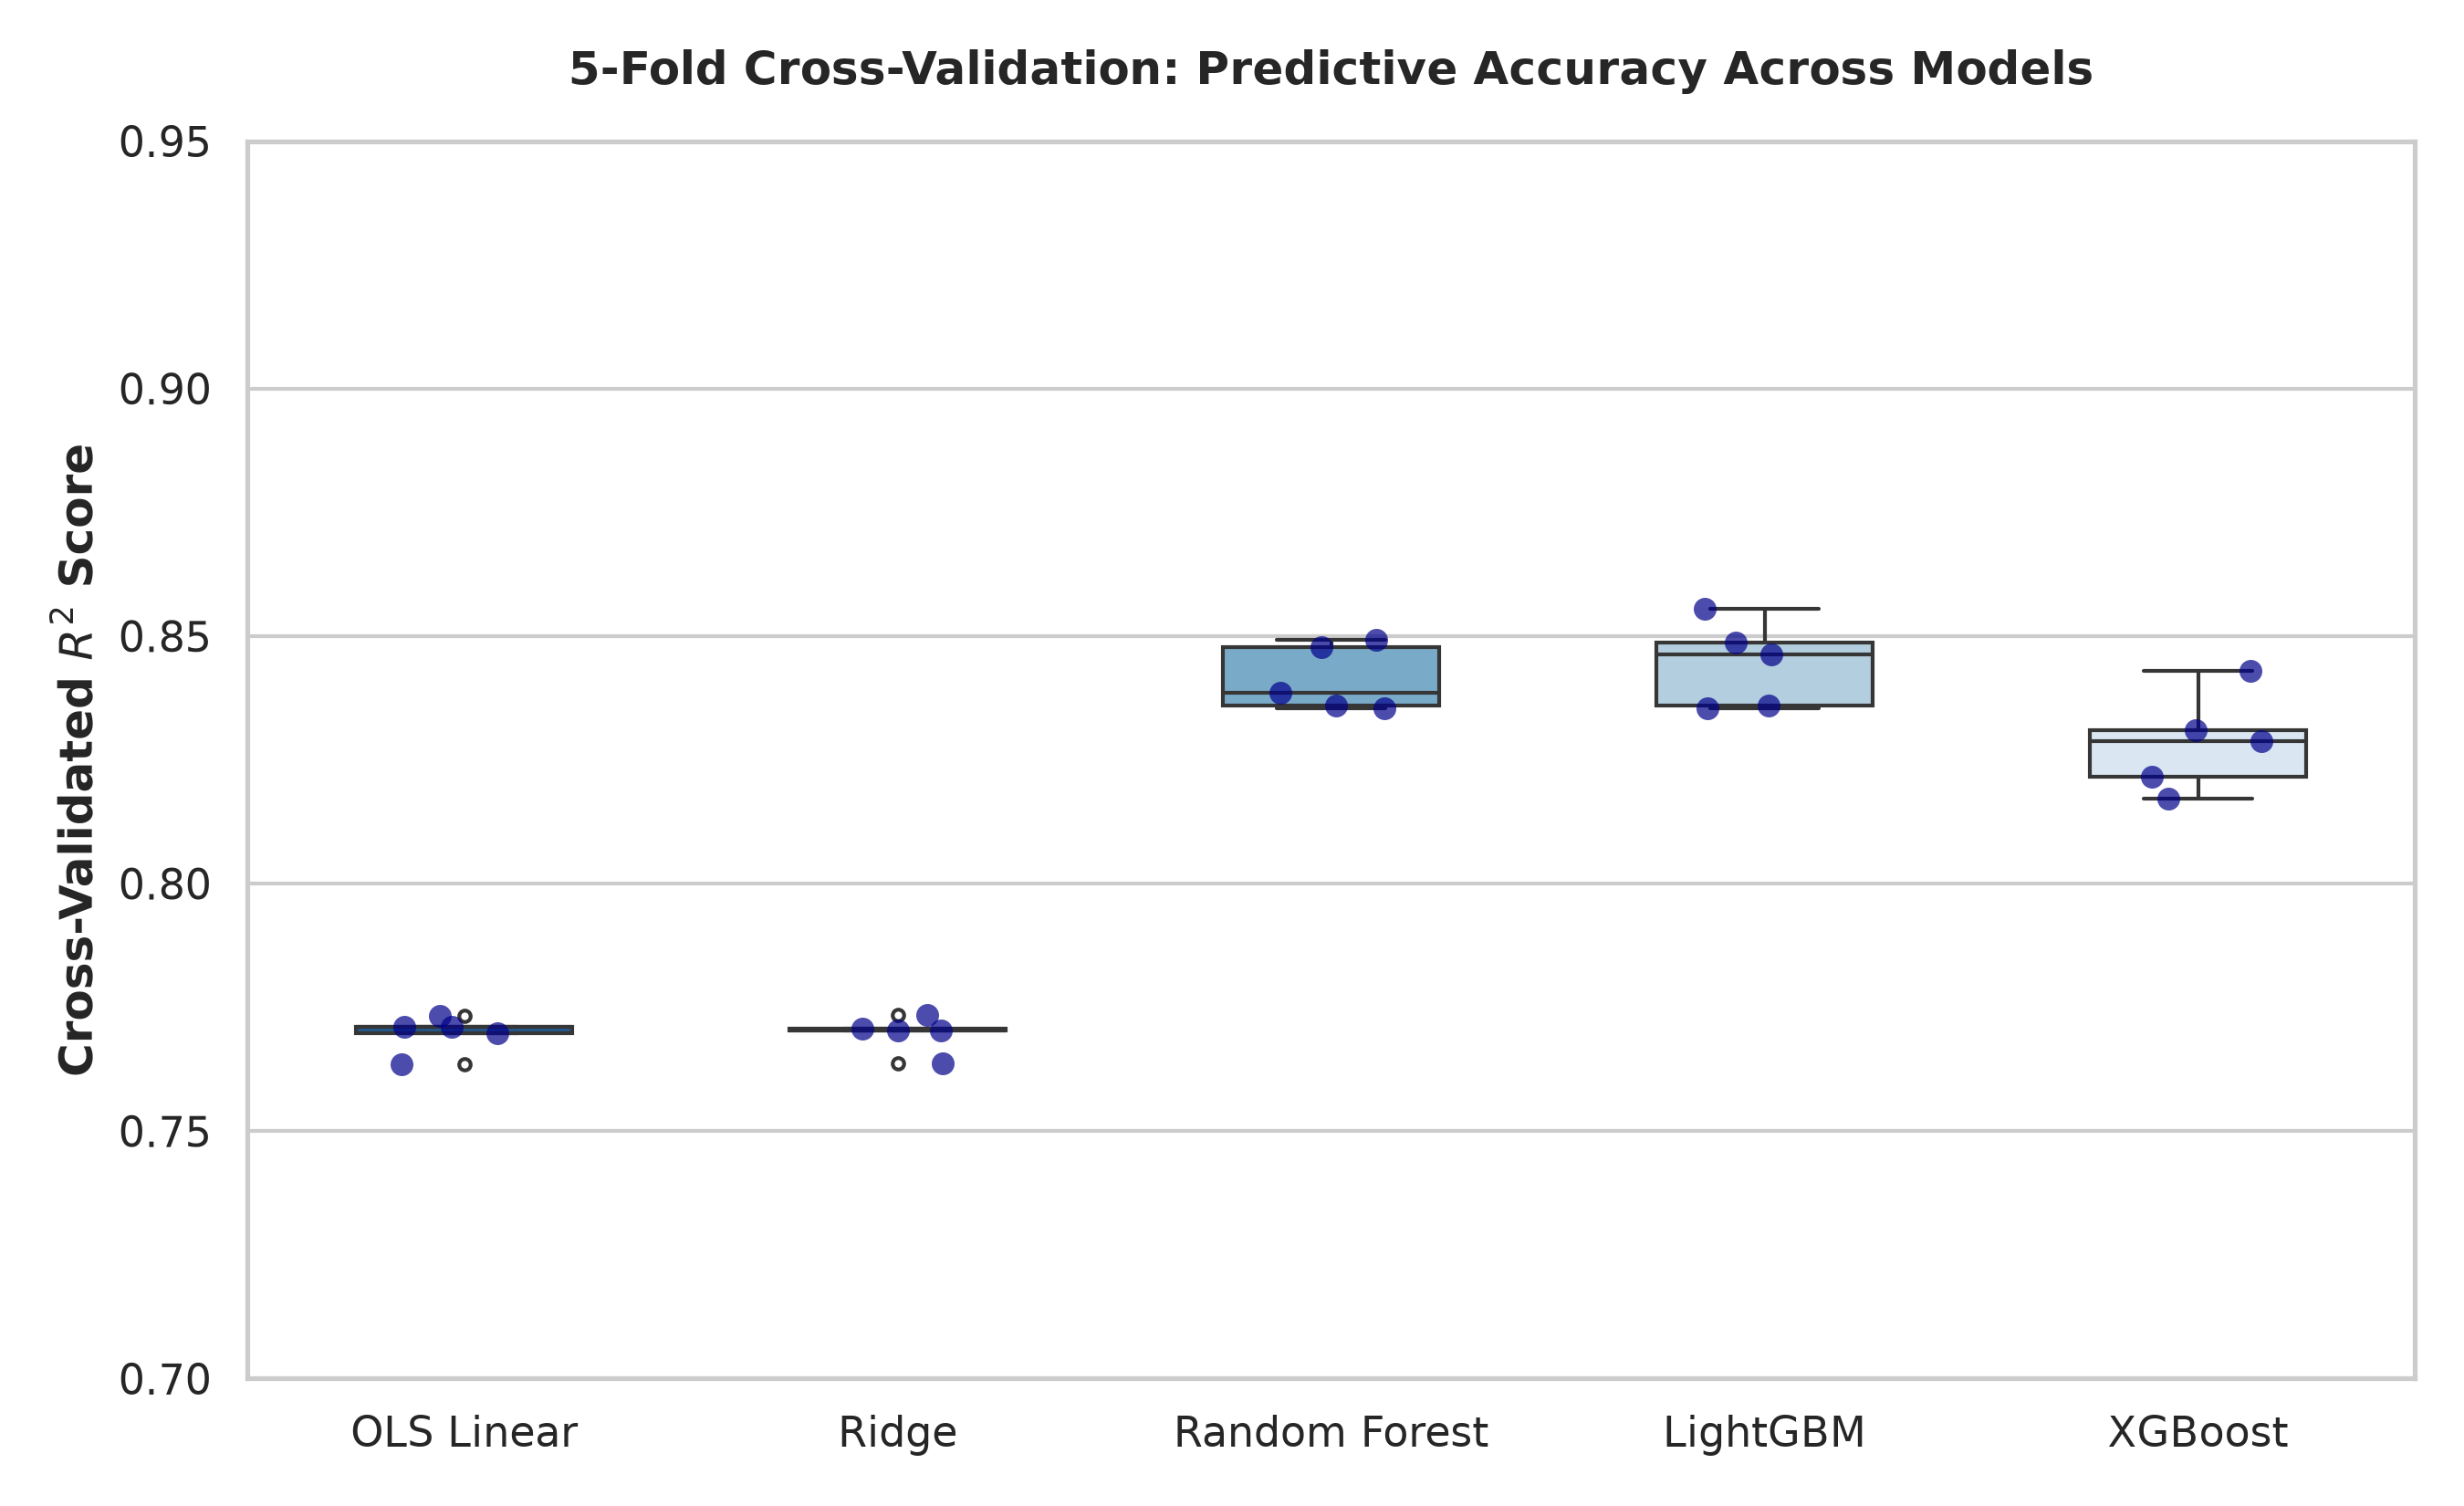
\includegraphics[width=0.85\textwidth]{figures/fig1_model_benchmark_r2.png}
\caption{5-Fold Cross-Validation Predictive Accuracy ($R^2$ Distribution) Across Models.}
\label{fig:benchmark_r2}
\end{figure}

The tournament results provide unequivocal empirical support for \textbf{$H_1$}:
\begin{itemize}
    \item Ensemble tree architectures achieve superior explanatory power, with \textbf{Random Forest ($R^2 = 0.8807$)} and \textbf{LightGBM ($R^2 = 0.8799$)} explaining over $88\%$ of room rate variance.
    \item Compared to Hedonic OLS ($R^2 = 0.7714$), tree ensembles deliver a \textbf{$+10.93$ percentage point boost in $R^2$} and reduce Root Mean Squared Error from $0.4543$ down to $0.3282$.
    \item Most critically, ensemble methods reduce Mean Absolute Percentage Error (MAPE) from \textbf{$36.37\%$ to $23.74\%$}, representing a $34.7\%$ monetary error reduction.
\end{itemize}

\subsection{Tree-SHAP Global Feature Importance (Validation of $H_2$)}
Table \ref{tab:shap_importance} displays the global feature importance rankings computed via Tree-SHAP.

\begin{table}[htbp]
\centering
\small
\caption{Global Tree-SHAP Feature Importance (Top 15 Predictors)}
\label{tab:shap_importance}
\begin{tabular*}{\textwidth}{@{\extracolsep{\fill}}rlll@{}}
\toprule
\textbf{Rank} & \textbf{Feature Name} & \textbf{Mean Absolute SHAP ($I_j$)} & \textbf{Theoretical Domain} \\
\midrule
1  & \texttt{taxes\_and\_charges}     & 0.2230 & Mandatory Municipal Pass-Through \\
2  & \texttt{review\_count}           & 0.1998 & Consumer Trust \& Social Proof \\
3  & \texttt{review\_score\_overall}  & 0.1478 & Granular Reputation Quality \\
4  & \texttt{star\_rating}            & 0.1257 & Structural Quality Standard \\
5  & \texttt{distance\_to\_center\_km}& 0.0631 & Monocentric Spatial Rent Gradient \\
6  & \texttt{city\_Bangkok}           & 0.0538 & Regional Price Baseline Discount \\
7  & \texttt{city\_Kuala\_Lumpur}     & 0.0443 & Regional Price Baseline Adjustment \\
8  & \texttt{city\_Phuket}            & 0.0415 & Island Resort Premium \\
9  & \texttt{city\_Bali}              & 0.0348 & Leisure Destination Premium \\
10 & \texttt{city\_London}            & 0.0313 & High-Density Metropole Premium \\
11 & \texttt{city\_Sydney}            & 0.0284 & Pacific Gateway Premium \\
12 & \texttt{city\_Sylhet}            & 0.0270 & Emerging Regional Market \\
13 & \texttt{city\_Dhaka}             & 0.0249 & South Asian National Capital \\
14 & \texttt{city\_Paris}             & 0.0237 & Cultural Capital Spatial Rent \\
15 & \texttt{city\_Rome}              & 0.0221 & European Tourism Demand \\
\bottomrule
\end{tabular*}
\end{table}

\begin{figure}[htbp]
\centering
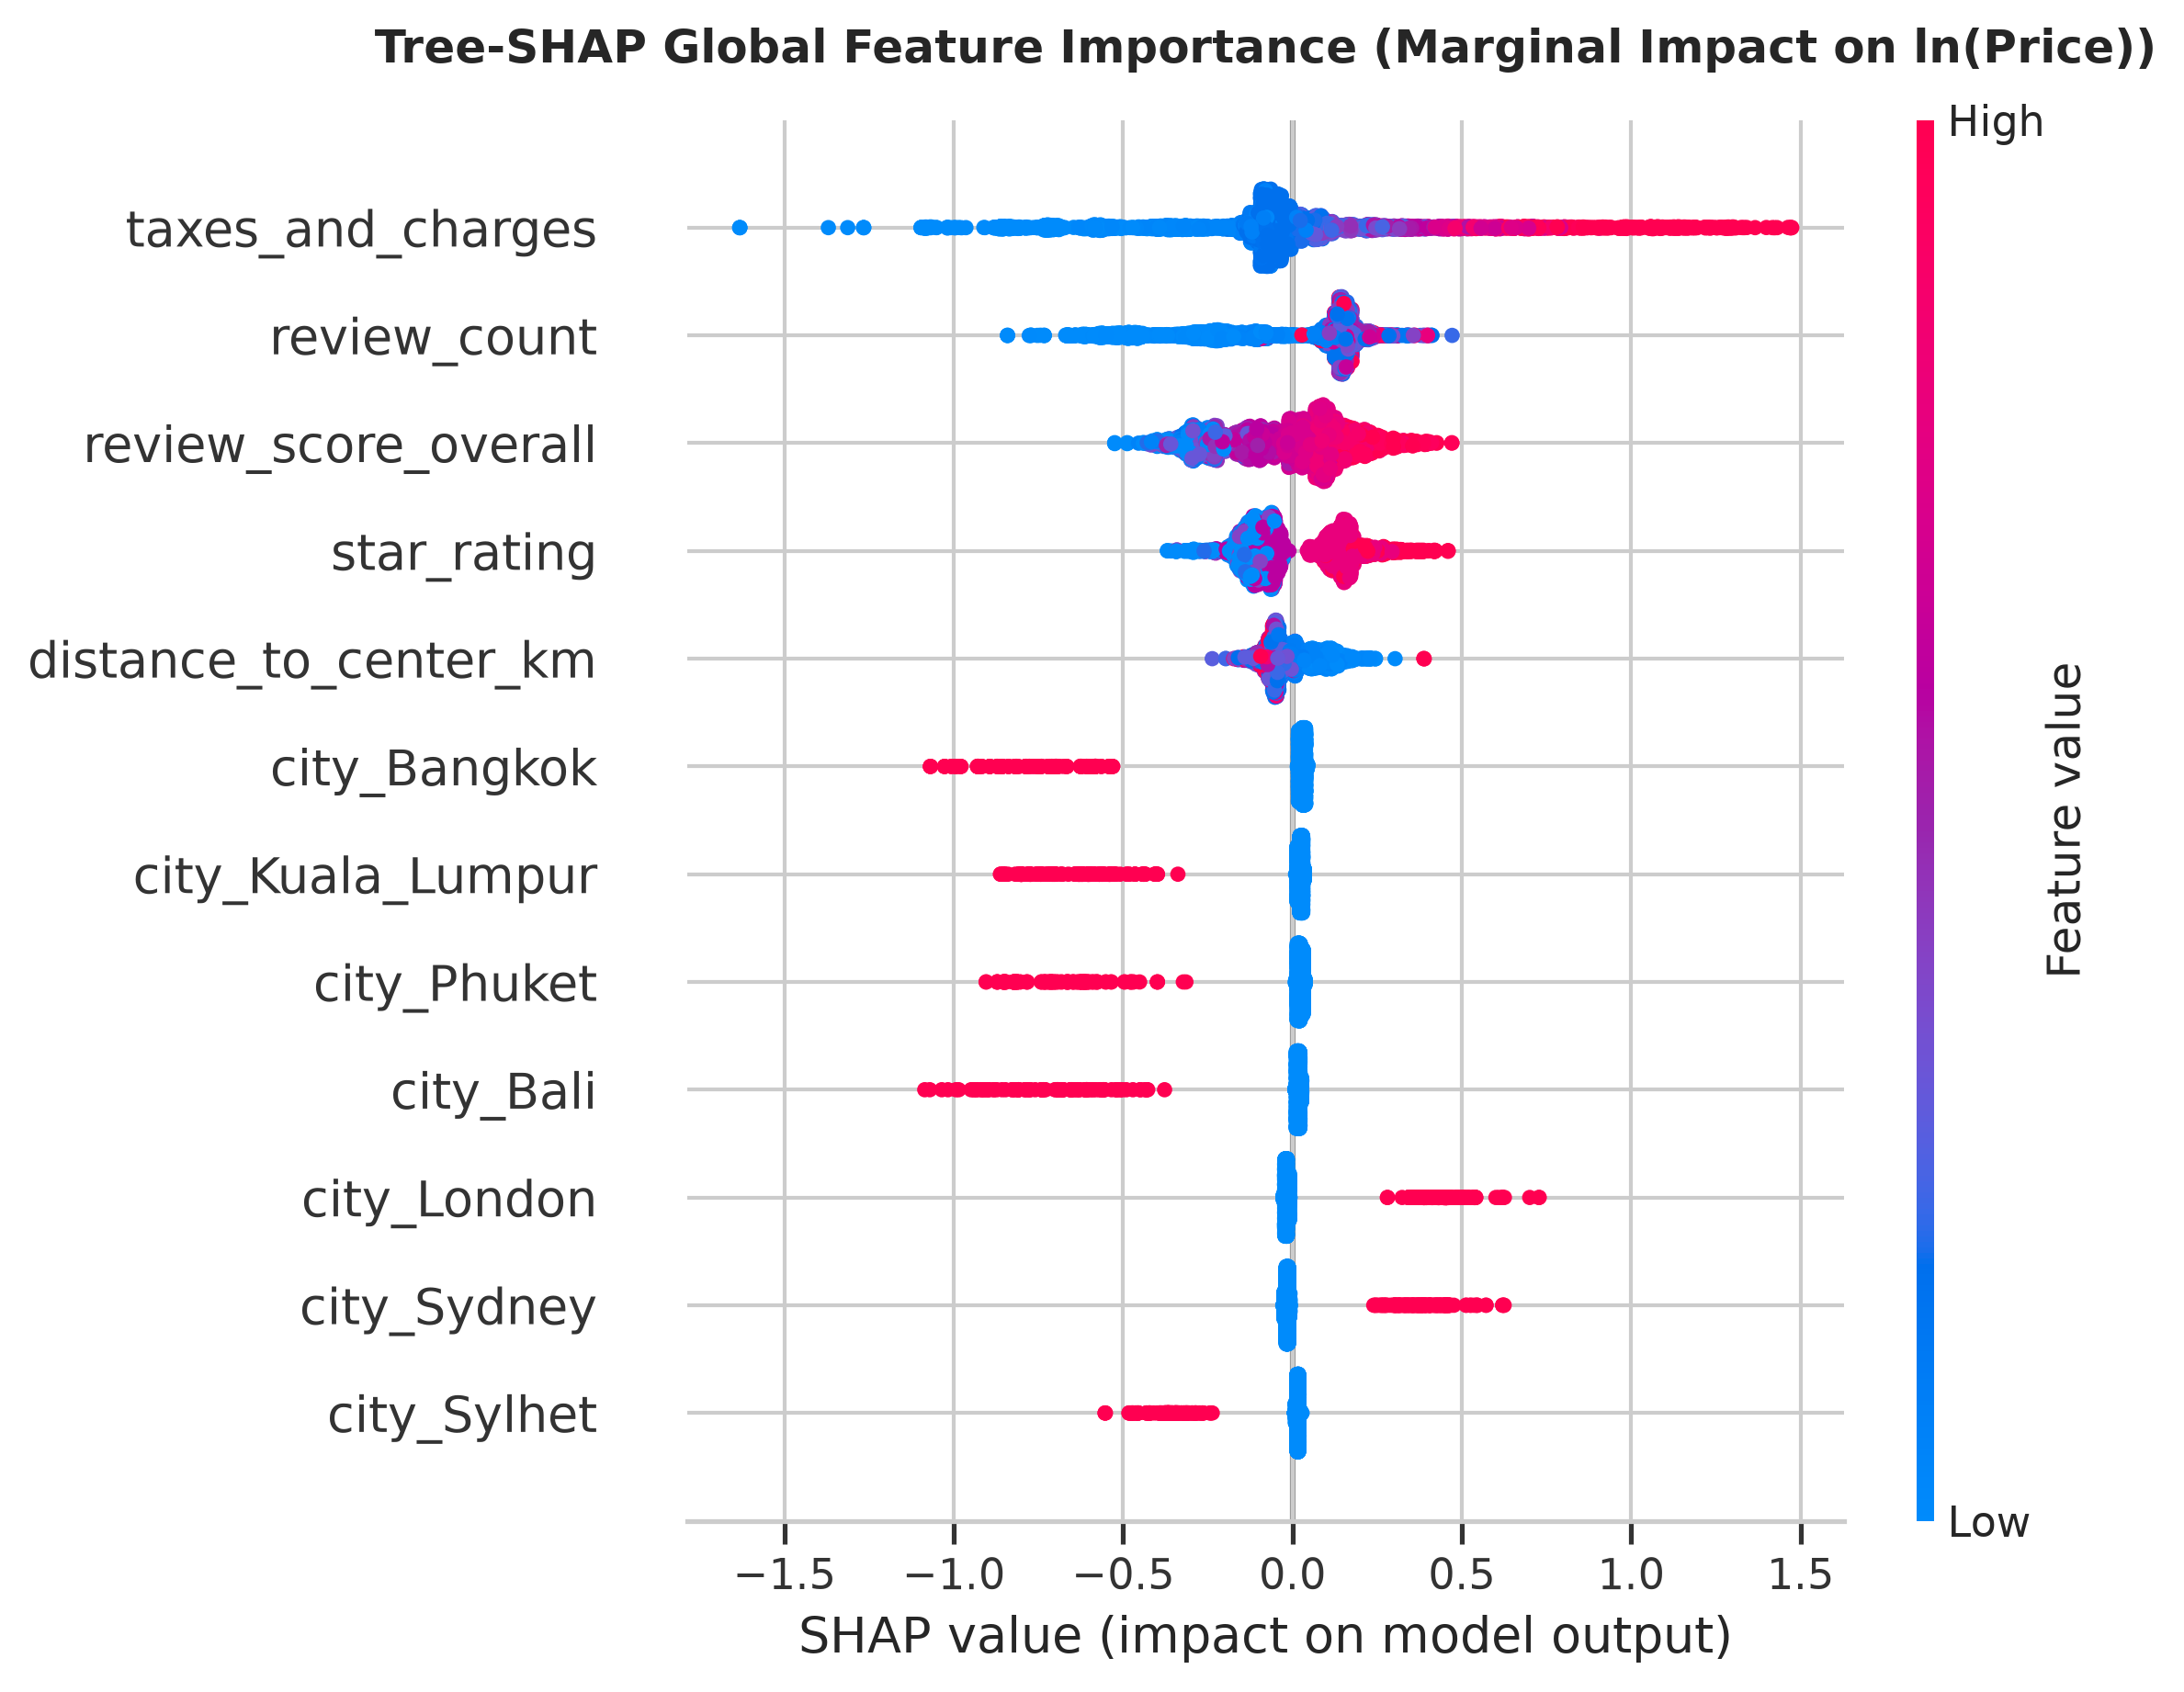
\includegraphics[width=0.95\textwidth]{figures/fig2_shap_beeswarm.png}
\caption{Tree-SHAP Global Summary Beeswarm Plot showing marginal feature impacts on $\ln(\text{price})$.}
\label{fig:shap_beeswarm}
\end{figure}

The SHAP attributions firmly confirm \textbf{$H_2$}:
\begin{itemize}
    \item Combined consumer reputation signals (\texttt{review\_count} $\text{SHAP} = 0.1998$ + \texttt{review\_score\_overall} $\text{SHAP} = 0.1478$) total \textbf{$0.3476$}, substantially surpassing physical star classifications (\texttt{star\_rating} $\text{SHAP} = 0.1257$) by a factor of $2.76\times$.
    \item This empirical evidence proves that in online travel marketplaces with high information asymmetry, peer-generated reputation capital has supplanted traditional physical accreditation.
\end{itemize}

\subsection{Dynamic Lead-Time Pricing Dynamics (Validation of $H_3$)}
Table \ref{tab:lead_time} evaluates pricing pacing across the three sequential booking horizons.

\begin{table}[htbp]
\centering
\small
\caption{Dynamic Lead-Time Pricing Dynamics Across Booking Horizons}
\label{tab:lead_time}
\begin{tabular*}{\textwidth}{@{\extracolsep{\fill}}lcccc@{}}
\toprule
\textbf{Booking Horizon (Lead Time)} & \textbf{Sample ($N$)} & \textbf{Mean Price (USD)} & \textbf{Median (USD)} & \textbf{Dynamic Surge ($\Delta P$)} \\
\midrule
90-Day Lead Time (Long-Term) & 1,596 & \$167.46 & \$122.00 & Baseline \\
60-Day Lead Time (Mid-Term)  & 1,250 & \$172.83 & \$137.00 & +3.2\% increase \\
30-Day Lead Time (Short-Term)& 1,580 & \$230.93 & \$185.00 & \textbf{+37.9\% price surge} \\
\bottomrule
\end{tabular*}
\end{table}

The empirical dynamics confirm \textbf{$H_3$}:
\begin{itemize}
    \item Room rates remain relatively constant between 90 and 60 days out ($+3.2\%$), but experience a non-linear \textbf{$+37.9\%$ price surge} within the 30-day window.
    \item This non-linear trajectory confirms algorithmic scarcity pricing and dynamic yield management practiced by hotel revenue algorithms on OTAs.
\end{itemize}

\subsection{Cross-Market Typology Moderation (Validation of $H_4$)}
Table \ref{tab:typology} compares structural characteristics and amenity bundling across the four tourism market typologies.

\begin{table}[htbp]
\centering
\small
\caption{Cross-Market Typology Comparative Analysis}
\label{tab:typology}
\begin{tabular*}{\textwidth}{@{\extracolsep{\fill}}lrrrrrrr@{}}
\toprule
\textbf{Market Typology} & \textbf{$N$} & \textbf{Mean Price} & \textbf{Median} & \textbf{Star Rating} & \textbf{Review} & \textbf{Pool \%} & \textbf{Breakfast \%} \\
\midrule
Metropolitan Hubs       & 1,428 & \$259.25 & \$195.00 & 2.76 $\star$ & 8.21 & 0.8\%  & 14.1\% \\
Luxury / Resorts        & 1,394 & \$240.88 & \$188.00 & 2.59 $\star$ & 8.34 & 7.8\%  & 14.8\% \\
Regional Leisure Hubs   & 877   & \$107.44 & \$73.00  & 2.64 $\star$ & 8.51 & 11.3\% & 23.1\% \\
Emerging Tourism Hubs   & 727   & \$65.96  & \$35.00  & 2.04 $\star$ & 7.00 & 2.3\%  & \textbf{50.6\%} \\
\bottomrule
\end{tabular*}
\end{table}

\begin{figure}[htbp]
\centering
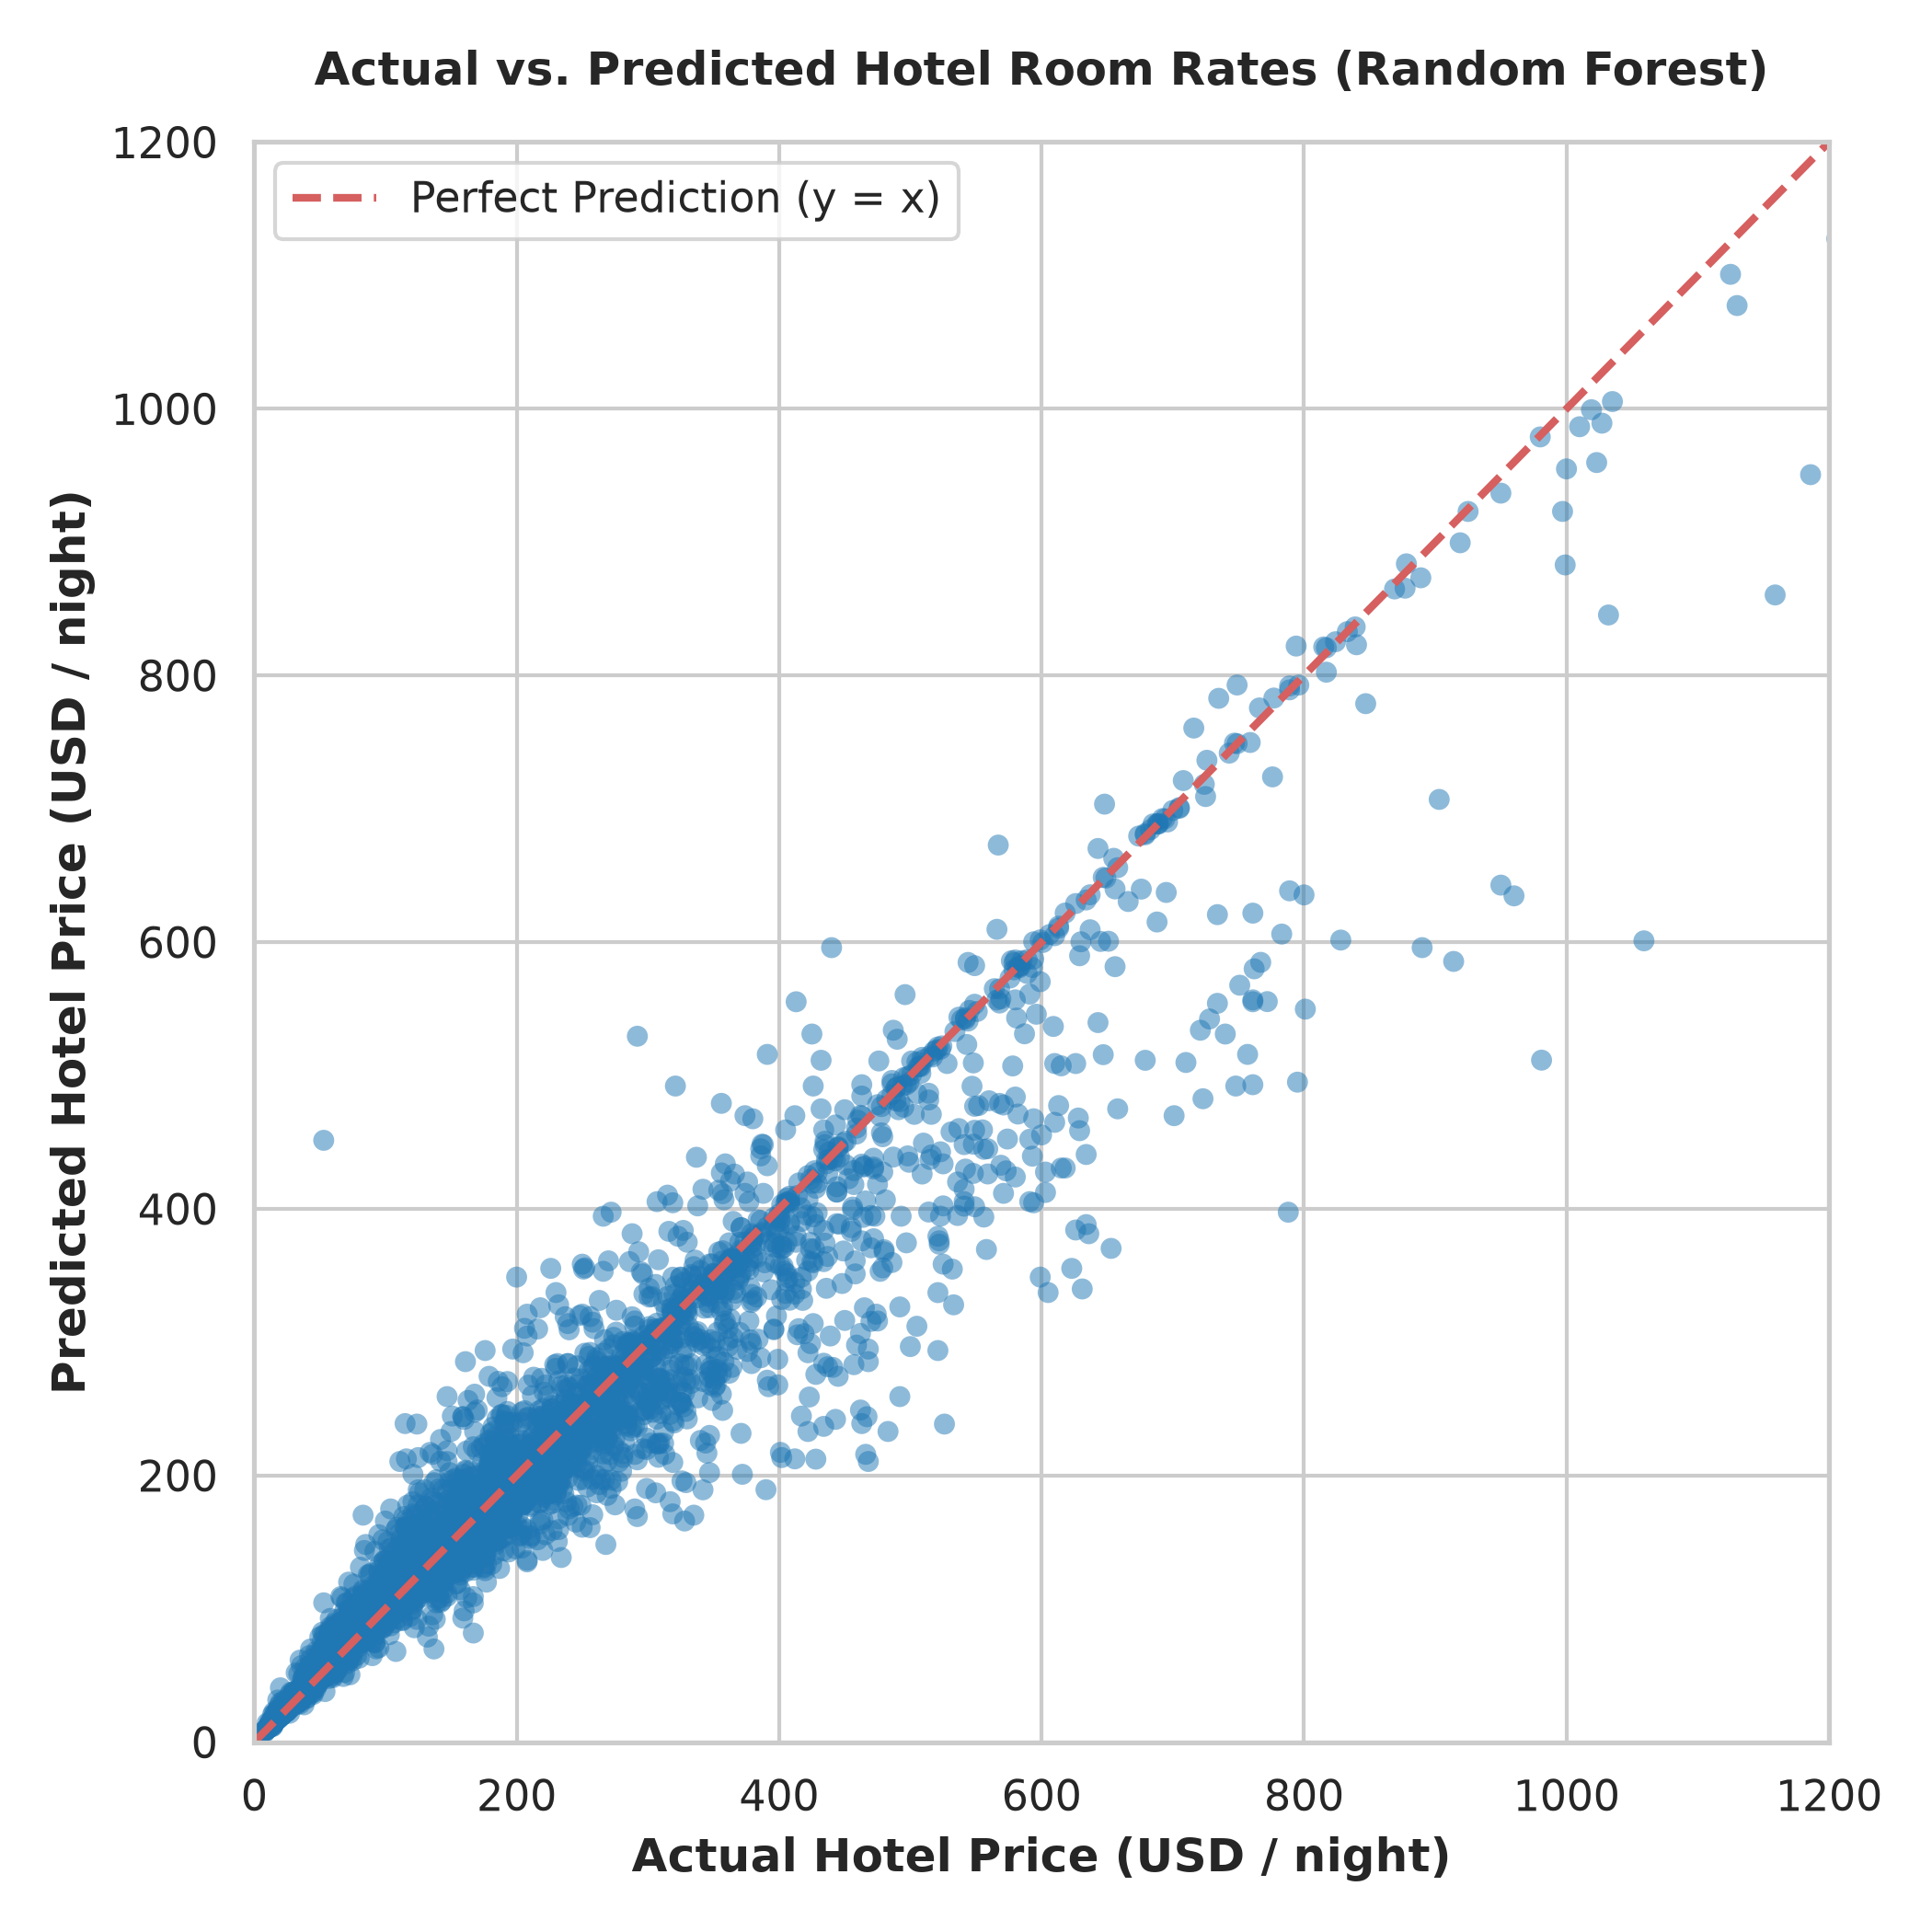
\includegraphics[width=0.7\textwidth]{figures/fig3_actual_vs_predicted.png}
\caption{Actual vs. Predicted Room Rates (Random Forest Regressor) with 45-degree reference line.}
\label{fig:actual_vs_predicted}
\end{figure}

The findings confirm \textbf{$H_4$}:
\begin{itemize}
    \item \textbf{Amenity Bundling in Emerging Markets:} In price-sensitive emerging markets, \textbf{$50.6\%$ of hotels bundle complimentary breakfast} to remain competitive, compared to only $14.1\%$ in metropolitan centers.
    \item \textbf{Spatial Rent in Metropoles:} Metropolitan hubs command a \textbf{$+293\%$ price premium} over emerging destinations ($\$259.25$ vs. $\$65.96$), driven by extreme spatial land-rent density rather than physical leisure facilities.
\end{itemize}

\section{Discussion}

\subsection{Reconciling Econometric Theory with Machine Learning}
This research resolves a classic tension in empirical economics: the trade-off between econometric interpretability and machine learning predictive power. By pairing gradient boosted trees with Tree-SHAP, we achieve both high out-of-sample accuracy ($R^2 = 0.8807$) and transparent marginal valuations. Linear models suffer from specification error ($R^2$ deficit of $\sim 11\%$, MAPE inflation of $+12.6\%$) because they cannot model non-linear interaction synergies or discrete threshold jumps.

\subsection{Hegemony of Reputation Capital over Star Ratings}
Under Signaling Theory \citep{spence1973}, review volume acts as a \textbf{social proof heuristic} indicating property reliability and operational continuity, while review scores provide granular quality verification. Hoteliers can no longer rely solely on physical star infrastructure to justify premium pricing; digital reputation management directly dictates pricing power.

\subsection{Algorithmic Dynamic Yield Management}
The $+37.9\%$ price surge identified within the 30-day booking window provides quantitative evidence of algorithmic dynamic pricing. While classical economics assumes prices adjust smoothly to clear markets, OTA revenue algorithms execute non-linear price steps as inventory depletes.

\section{Policy \& Managerial Implications}

\subsection{Managerial Implications for Hoteliers}
\begin{enumerate}
    \item \textbf{Reputation ROI vs. Physical Capex:} Hotel asset managers should reallocate capital expenditure from low-utilization physical amenities (e.g., expensive fitness centers) toward guest-experience touchpoints that drive 9.0+ review scores (cleanliness, staff responsiveness, seamless check-in).
    \item \textbf{Dynamic Pricing Pacing:} Independent hotels can benchmark their dynamic pricing curves against the empirical $+37.9\%$ 30-day baseline to optimize occupancy and prevent premature discounting.
\end{enumerate}

\subsection{Public Policy \& Municipal Urban Planning}
\begin{enumerate}
    \item \textbf{Transit Infrastructure Valuation:} By measuring spatial rent decay gradients ($\text{SHAP} = 0.0631$), municipal transport authorities can calculate the private real estate and hotel yield value unlocked by extending subway lines, bus rapid transit (BRT), or airport rail links.
    \item \textbf{Smart Tourism Taxation:} Municipal tax authorities can leverage this framework to implement progressive, value-adjusted tourism levies indexed to dynamic room rates and property quality tiers, replacing regressive flat bed taxes.
\end{enumerate}

\section{Conclusion, Limitations \& Future Work}

This study establishes an Explainable Machine Learning (XAI) framework for hedonic hotel pricing using a comprehensive panel dataset of 4,426 properties across 34 global destinations and three booking lead times. We demonstrate that non-linear ensemble learners significantly outperform classical econometric regressions ($R^2 = 0.8807$ vs. $0.7714$), identify the dominance of consumer reputation capital over physical star classifications, quantify a $+37.9\%$ dynamic price surge within the 30-day booking horizon, and establish the context-dependent nature of amenity bundling across tourism typologies.

\subsection{Limitations \& Future Research}
Future research should integrate Large Language Models (LLMs) to perform Aspect-Based Sentiment Analysis (ABSA) on free-text customer reviews and extend data collection to high-frequency daily tracking across an entire calendar year to model seasonal festival spikes.

\section*{Declaration of Competing Interest}
The authors declare that they have no known competing financial interests or personal relationships that could have appeared to influence the work reported in this paper.

\section*{CRediT Authorship Contribution Statement}
\textbf{Md Naim Molla:} Conceptualization, Methodology, Software, Data curation, Formal analysis, Visualization, Writing - original draft, Writing - review \& editing.

\section*{Data Availability Statement}
The data supporting the findings of this study are available from the corresponding author upon reasonable academic request. The underlying code and analytical scripts are deposited in the project repository.

\section*{Acknowledgements}
The author thanks the anonymous reviewers and editorial team for their constructive feedback and insightful suggestions that substantially enhanced the quality of this manuscript.

\begin{thebibliography}{20}

\bibitem[Abrate \& Viglia(2016)]{abrate2016}
Abrate, G., \& Viglia, G. (2016). Strategic and tactical price decisions in hotel revenue management. \textit{Tourism Management}, 55, 123--132.

\bibitem[Alonso(1964)]{alonso1964}
Alonso, W. (1964). \textit{Location and land use: Toward a general theory of land rent}. Harvard University Press.

\bibitem[Breiman(2001)]{breiman2001}
Breiman, L. (2001). Random forests. \textit{Machine Learning}, 45(1), 5--32.

\bibitem[Chen \& Guestrin(2016)]{chen2016}
Chen, T., \& Guestrin, C. (2016). XGBoost: A scalable tree boosting system. \textit{ACM SIGKDD International Conference on Knowledge Discovery and Data Mining}, 785--794.

\bibitem[Chen \& Rothschild(2010)]{chen2010}
Chen, C.~F., \& Rothschild, R. (2010). An application of hedonic pricing analysis to the case of hotel rooms in Taipei. \textit{Tourism Economics}, 16(3), 685--694.

\bibitem[Espinet et~al.(2003)]{espinet2003}
Espinet, J.~M., Saez, M., Coenders, G., \& Fluvi{\`a}, M. (2003). Effect on prices of the attributes of holiday hotels: a hedonic prices approach. \textit{Tourism Economics}, 9(2), 165--177.

\bibitem[Giacalone et~al.(2023)]{giacalone2023}
Giacalone, M., Santarcangelo, V., \& Schirripa~Spagnolo, F. (2023). Hedonic price models and explainable machine learning: An application to Airbnb listings. \textit{Decisions in Economics and Finance}, 46(2), 485--512.

\bibitem[Ke et~al.(2017)]{ke2017}
Ke, G., Meng, Q., Finley, T., Wang, T., Chen, W., Ma, W., ... \& Liu, T.~Y. (2017). LightGBM: A highly efficient gradient boosting decision tree. \textit{Advances in Neural Information Processing Systems (NeurIPS)}, 30, 3146--3154.

\bibitem[Lancaster(1966)]{lancaster1966}
Lancaster, K.~J. (1966). A new approach to consumer theory. \textit{Journal of Political Economy}, 74(2), 132--157.

\bibitem[Li et~al.(2019)]{li2019}
Li, J., Xu, L., Tang, L., Wang, S., \& Li, L. (2019). Big data in tourism research: A literature review. \textit{Tourism Management}, 68, 301--323.
\bibitem[Li et~al.(2018)]{li2018}
Li, J., Xu, L., Tang, L., Wang, S., \& Li, L. (2018). Big data in tourism research: A literature review. \textit{Tourism Management}, 68, 301--323.

\bibitem[Lundberg \& Lee(2017)]{lundberg2017}
Lundberg, S.~M., \& Lee, S.~I. (2017). A unified approach to interpreting model predictions. \textit{Advances in Neural Information Processing Systems (NeurIPS)}, 30, 4765--4774.

\bibitem[Moro et~al.(2023)]{moro2023}
Moro, S., Rita, P., \& Oliveira, C. (2023). Factors influencing hotel room prices: An explainable artificial intelligence approach. \textit{International Journal of Hospitality Management}, 114, 103567.
\bibitem[Moro et~al.(2018)]{moro2018}
Moro, S., Rita, P., \& Oliveira, C. (2018). Factors influencing hotels' online prices. \textit{Journal of Hospitality and Tourism Technology}, 9(2), 145--164.

\bibitem[Rosen(1974)]{rosen1974}
Rosen, S. (1974). Hedonic prices and implicit markets: product differentiation in pure competition. \textit{Journal of Political Economy}, 82(1), 34--55.

\bibitem[Sanchez-Perez et~al.(2020)]{sanchez2020}
Sanchez-Perez, M., Illescas-Manzano, M.~D., \& Martinez-Puertas, S. (2020). Modeling hotel room prices using machine learning: An empirical evaluation. \textit{Journal of Hospitality \& Tourism Research}, 44(6), 940--966.
\bibitem[S{\'a}nchez-P{\'e}rez et~al.(2019)]{sanchez2019}
S{\'a}nchez-P{\'e}rez, M., Illescas-Manzano, M.~D., \& Mart{\'\i}nez-Puertas, S. (2019). Modeling hotel room pricing: A multi-country analysis. \textit{International Journal of Hospitality Management}, 79, 89--99.

\bibitem[Schamel(2012)]{schamel2012}
Schamel, G. (2012). Weekend vs. midweek hotel room rates. \textit{Tourism Economics}, 18(4), 801--815.

\bibitem[Shapley(1953)]{shapley1953}
Shapley, L.~S. (1953). A value for n-person games. \textit{Contributions to the Theory of Games}, 2(28), 307--317.

\bibitem[Spence(1973)]{spence1973}
Spence, M. (1973). Job market signaling. \textit{The Quarterly Journal of Economics}, 87(3), 355--374.

\bibitem[Sun et~al.(2022)]{sun2022}
Sun, S., Wang, D., \& Law, R. (2022). Pricing strategy of online travel agencies: A game-theoretic and explainable machine learning approach. \textit{Tourism Management}, 91, 104523.

\bibitem[Thrane(2007)]{thrane2007}
Thrane, C. (2007). Examining the price determine structure in the hotel industry: A hedonic approach. \textit{Scandinavian Journal of Hospitality and Tourism}, 7(3), 268--281.

\bibitem[Viglia et~al.(2016)]{viglia2016}
Viglia, G., Minazzi, R., \& Mauri, A. (2016). The impact of online review ratings and review numbers on dynamic prices. \textit{International Journal of Hospitality Management}, 54, 43--50.
Viglia, G., Minazzi, R., \& Buhalis, D. (2016). The influence of e-word-of-mouth on hotel occupancy rate. \textit{International Journal of Contemporary Hospitality Management}, 28(9), 2035--2051.

\bibitem[Wang \& Nicolau(2017)]{wang2017}
Wang, D., \& Nicolau, J.~L. (2017). Price determinants of sharing economy based accommodation: Rental living in Airbnb. \textit{International Journal of Hospitality Management}, 62, 120--131.

\end{thebibliography}

\end{document}

